Fig. \ref{fig:ad7} shows a comparison on the support vector growth on two
standard benchmark databases\footnote{Available at
\url{http://www.csie.ntu.edu.tw/~cjlin/libsvmtools/datasets}}. For
each benchmark, data are obtained by running $10$ random $75\%$/$25\%$
train/test runs. Consider Fig. \ref{fig:ad7}, left panel, Diabetes dataset. When all
samples have been loaded, LIBSVM2 has about $427$ SVs, and IncrSVM
about $290$. The kernel used is a homogeneous polynomial with degree
$3$ and the benchmark has $8$ features, therefore the dimension of the
feature space is $\binom{10}{3} = 120$ \cite{Cristianini00};
as expected, OISVM stops acquiring new SVs when there are exactly
$120$, although it loads a few more than the other approaches before
reaching the limit. The accuracy (not displayed) is exactly the
same of LIBSVM2. On the other hand, the size of the solutions of
IncrSVM and LIBSVM2 will grow beyond the strict necessary $120$ vectors,
as theoretically proved in \cite{Steinwart03}.

Consider now Fig. \ref{fig:ad7}, right panel, Adult7 dataset. The
kernel used is Gaussian and its dimension is infinite. The benchmark
is large and complex ($16100$ samples, $123$ features); nevertheless,
with $\eta=0.1$, at the end OISVM has about $2\%$ of the SVs used by
LIBSVM2 and less than $4\%$ with respect to IncrSVM. The accuracy is
essentially the same as that of LIBSVM2 (namely, an absolute loss of
accuracy of $0.069\%\pm0.068$). In Fig. \ref{fig:sv_cr} there is a graph
showing the accuracy as a function of the number of basis vectors.
It is clear that OISVM reaches better performance with less basis vectors,
with respect to IncrSVM and LIBSVM2.

Lastly, consider Table \ref{table:t1}, which shows the very same results
in compact form for $10$ more databases. In each column we
show the mean recognition rate on 10 train/test splits taken from
\cite{Ratsch05}, and the number of support vectors in parenthesis. We
have compared our method to the batch method LIBSVM2 and to IncrSVM.
Cross validation was used to find the best parameters for each dataset,
separately for the norm-1 and norm-2 formulation, while for OISVM we used the same
parameters of the norm-2. OISVM attains a number of SVs which is
from about $3$ to slightly more than $60$ times less than LIBSVM2, whereas
the accuracy is not worse than $0.5\%$. Moreover it is always sparser
than the norm-1 formulation.

\begin{figure*}[t]
  \centering \footnotesize
  \begin{tabular}{cc}
  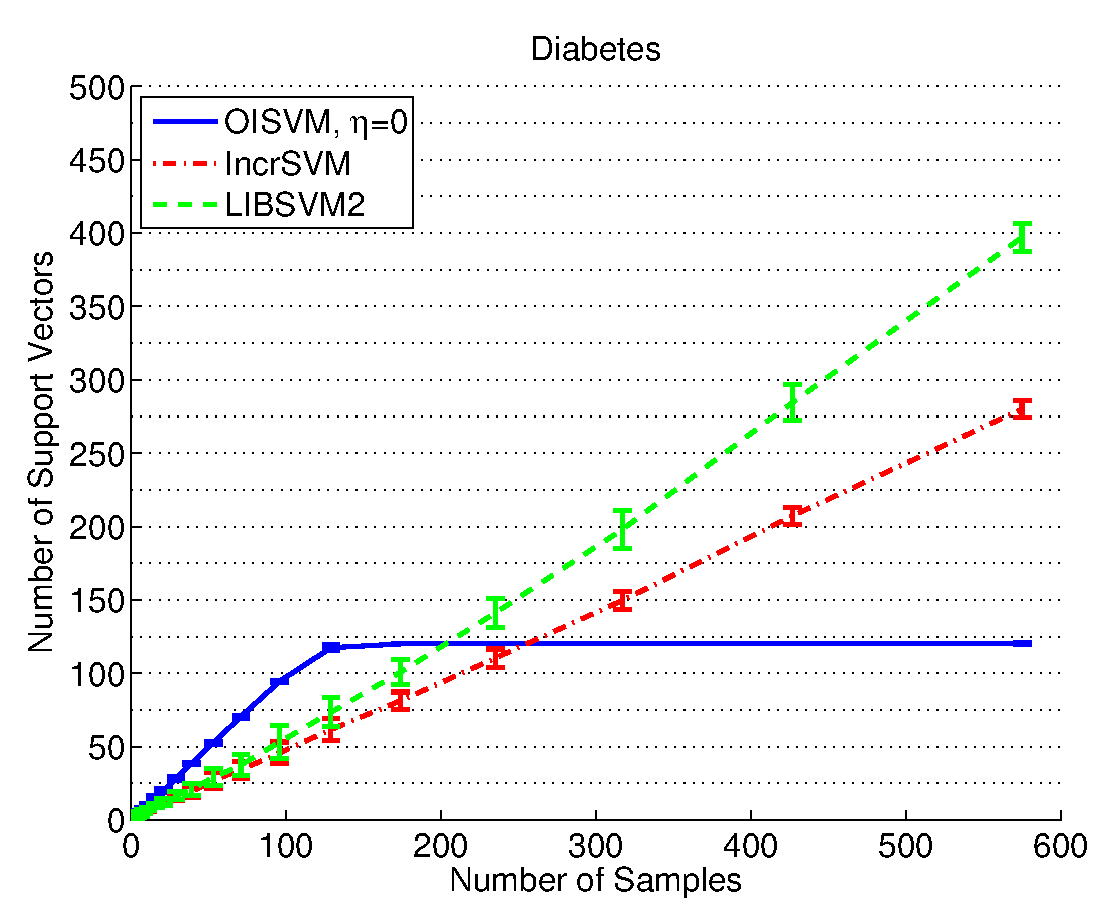
\includegraphics[width=0.48\linewidth]{figs/results/diabetis_sv} &
  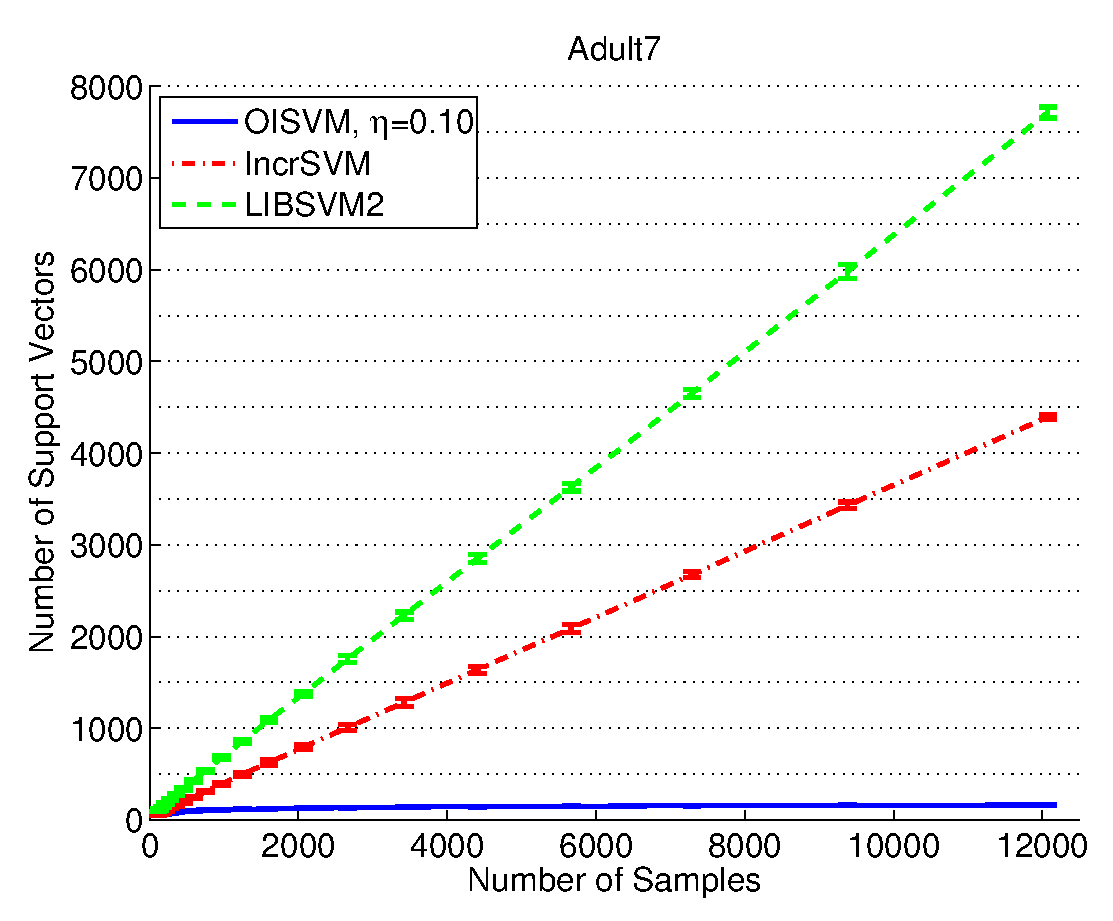
\includegraphics[width=0.48\linewidth]{figs/results/adult7_sv} 
  \end{tabular}
  \caption{Comparison of LIBSVM2, IncrSVM and OISVM and on the \emph{Diabetes}
  (left panel) and \emph{Adult7} (right panel) benchmarks.
  \emph{Diabetes} is solved using a polynomial kernel with degree $3$,
  while \emph{Adult7} is solved using a Gaussian kernel.}
\label{fig:ad7}
\end{figure*}

\begin{figure*}[t]
  \centering \footnotesize
  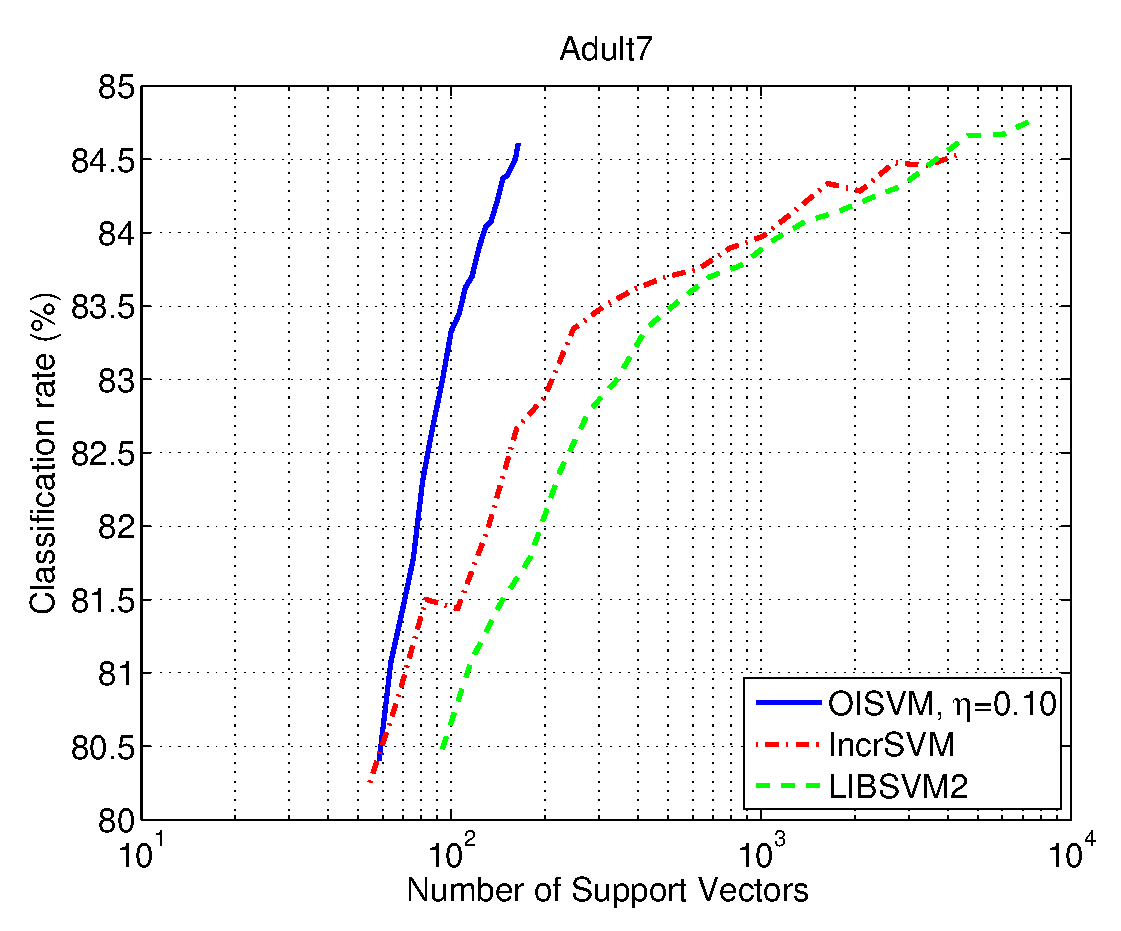
\includegraphics[width=0.48\linewidth]{figs/results/adult7_sv_cr}
  \caption{Comparison of LIBSVM2, IncrSVM and OISVM on the \emph{Adult7} dataset.}
\label{fig:sv_cr}
\end{figure*}

\begin{table}[t]
\tiny
\renewcommand{\arraystretch}{1.3}
\caption{Comparison of OISVM, RSVM, IncrSVM and LIBSVM2 on 10 standard benchmarks, solved
 using a Gaussian kernel. For each benchmark, we report the classification rate and
 the number of SVs. The value of $\eta$ has been chosen in order not to loose
 more than $0.5\%$ accuracy with respect to LIBSVM2.}
\label{table:t1}
\centering
\begin{tabular}[!h]{lcccc}
\hline
    Dataset   & OISVM                           & RSVM           & LIBSVM2                          & IncrSVM                            \\ \hline
     Banana   & $89.54\pm0.41$ ($18.90\pm1.29$) & $88.81\pm0.63$ & $89.75\pm0.30$ ($173.60\pm21.20$) & $89.77\pm0.28$ ($121.10\pm9.01$)  \\
     Breast   & $73.51\pm4.21$ ($36.00\pm2.67$) & $71.95\pm4.79$ & $74.03\pm4.15$ ($199.70\pm0.67$)  & $74.55\pm4.16$ ($122.60\pm4.95$)  \\
     Diabetis & $76.83\pm2.13$ ($8.60\pm0.52$)  & $75.77\pm2.85$ & $76.83\pm2.21$ ($417.00\pm4.00$)  & $76.83\pm1.77$ ($283.30\pm8.17$)  \\
     Flare    & $66.35\pm1.17$ ($10.40\pm0.70$) & $63.77\pm4.05$ & $66.35\pm1.23$ ($631.10\pm4.20$)  & $67.15\pm1.63$ ($555.70\pm8.59$)  \\
     German   & $76.20\pm1.93$ ($52.60\pm2.46$) & $75.43\pm2.20$ & $76.70\pm1.79$ ($600.70\pm11.89$) & $76.37\pm2.60$ ($384.70\pm7.01$)  \\
     Heart    & $84.90\pm1.91$ ($14.30\pm0.67$) & $84.30\pm2.95$ & $85.00\pm1.83$ ($161.60\pm2.63$)  & $85.00\pm2.87$ ($85.00\pm3.27$)   \\
     Ringnorm & $98.03\pm0.27$ ($87.60\pm6.01$) & $98.60\pm0.10$ & $98.57\pm0.10$ ($377.00\pm4.06$)  & $98.50\pm0.10$ ($213.00\pm4.74$)  \\
     Titanic  & $77.84\pm0.66$ ($11.90\pm1.37$) & $74.81\pm3.24$ & $77.60\pm1.63$ ($146.00\pm5.27$)  & $77.28\pm0.35$ ($86.80\pm6.91$)   \\
     Twonorm  & $97.14\pm0.34$ ($60.60\pm5.44$) & $97.18\pm0.32$ & $97.44\pm0.26$ ($400.00\pm0.00$)  & $97.65\pm0.09$ ($299.90\pm5.74$)  \\
     Waveform & $89.67\pm0.47$ ($78.20\pm3.12$) & $89.66\pm0.65$ & $90.10\pm0.36$ ($324.60\pm9.43$)  & $89.62\pm0.58$ ($220.30\pm10.49$) \\ \hline
\end{tabular}
\end{table}

For a complete comparison we have used also a variation of the Reduced
Support Vector Machine (RSVM) method \cite{LeeM01}, the same used also
in \cite{KeerthiCDC06}, in which for each run we have randomly
selected a number of basis vectors equal to the one selected by
OISVM. In this way we compare the two methods with the same number
of basis vectors. We have used a Wilcoxon signed-ranks test to compare the
performances of the two methods, as suggested in \cite{Demsar06},
obtaining a p-value less than $0.02$. This confirms that our strategy
to select basis vectors is better than the random sampling,
suggested by many authors, e.g. \cite{RifkinYP03}. As a plus our
strategy assures that, as said before, the growth of basis vectors
will always eventually stop.

To gain more understanding on the difference between RSVM and OISVM we
have also compared the value of the objective function
(\ref{eqn:svm_primal}) at the end of each dataset. The results are in
Table \ref{table:t1_o}, where the relative difference between the
value of the objective function of OISVM and RSVM compared to LIBSVM2
are shown. There is a clear correlation between good classification
accuracy and good value of the objective function. Hence our method
seems to select the basis vectors in a way that allows a better
minimization of (\ref{eqn:svm_primal}). This can be explained
intuitively noting that adding a linearly dependent vector to the basis
set will not help in minimizing the objective function.
The negative result on \emph{Ringnorm} is somehow surprising given the corresponding
good classification performance, but it should not worry as
the value of the objective function is loosely related to the classification performance.
Hence the big increment in the objective function does not necessarily
correspond to very bad classification performance, as it is shown
in Table \ref{table:t1}.

We have also conducted other experiments to compare the speed of the
algorithms. Given that our implementation is in Matlab, so not optimized for
speed, to have a fair comparison we have considered the number of kernel
evaluations as a figure of merit. This is a standard measure
for an implementation invariant comparison\footnote{However note that our Matlab implementation
of OISVM is about 1 order of magnitude faster than the Matlab implementation of IncrSVM.},
see for example \cite{BordesEWB05,DiehlC03}.
We have used 3 databases, \emph{Adult7}, \emph{Banana} and \emph{Waveform}, with
the same kernel and parameters used in \cite{BordesEWB05}. 
In Fig. \ref{fig:kernel_eval} we show the performance on the test set
as a function of the number of kernel evaluations. For LIBSVM2 and IncrSVM we have just
a point on the graph, while for OISVM we have a curve obtained varying $\eta$\footnote{
The values of $\eta$ for the 3 datasets are respectively $[0.4;0.3;0.2;0.1;0.05;0.01],
[0.7;0.6;0.5;0.4;0.3;0.2;0.1;0.01],[0.8;0.7;0.6;0.5;0.4;0.3]$.}.
In other words, in OISVM we can trade accuracy for training (and testing) speed.
From the figure we can see that OISVM achieves better or comparable performance
to the other methods with much less kernel computations. Moreover the degree of freedom
given by the sparsification method allows to trade just 0.5\% of performance to
save more than 1 order of magnitude of kernel computations.
Note that the accuracy of OISVM is not always monotonically increasing with
$\eta$ going to 0. A possible explanation is that the sparsification procedure
can be seen as a form of regularization; a similar view has been proposed in 
\cite{BlanchardMVZ05}. Hence it is plausible to suppose that there is an optimal
value of $\eta$ that gives better generalization properties.

\begin{table}
%\renewcommand{\arraystretch}{1.3}
\caption{Loss in percentage of the objective function of OISVM and RSVM in relation to the one
 of LIBSVM2 on 10 standard benchmarks, solved using a Gaussian kernel. The values of $\eta$
 are the same of Table \ref{table:t1}.}
\label{table:t1_o}
\centering
\footnotesize
\begin{tabular}[!h]{lcccc}
\hline
    Dataset   & OISVM          & RSVM            \\ \hline
     Banana   & $13.9\pm3.2$ & $23.5\pm10.5$ \\
     Breast   & $2.1\pm0.4$  & $3.3\pm0.4$   \\
     Diabetis & $1.7\pm1.2$  & $3.8\pm4.7$   \\
     Flare    & $0.1\pm0$    & $4.6\pm6.3$   \\
     German   & $9.7\pm1.4$  & $9.9\pm0.5$   \\
     Heart    & $0.9\pm0.3$  & $1.5\pm1.0$   \\
     Ringnorm & $43.0\pm4.6$ & $3.6\pm0.4$   \\
     Titanic  & $0\pm0$      & $15.8\pm10.8$ \\
     Twonorm  & $5.6\pm0.8$  & $8.9\pm1.0$   \\
     Waveform & $10.4\pm0.6$ & $10.4\pm1.0$  \\ \hline
\end{tabular}
\end{table}

\begin{figure*}[!ht]
  \centering \footnotesize
  \begin{tabular}{cc}
  \multicolumn{2}{c}{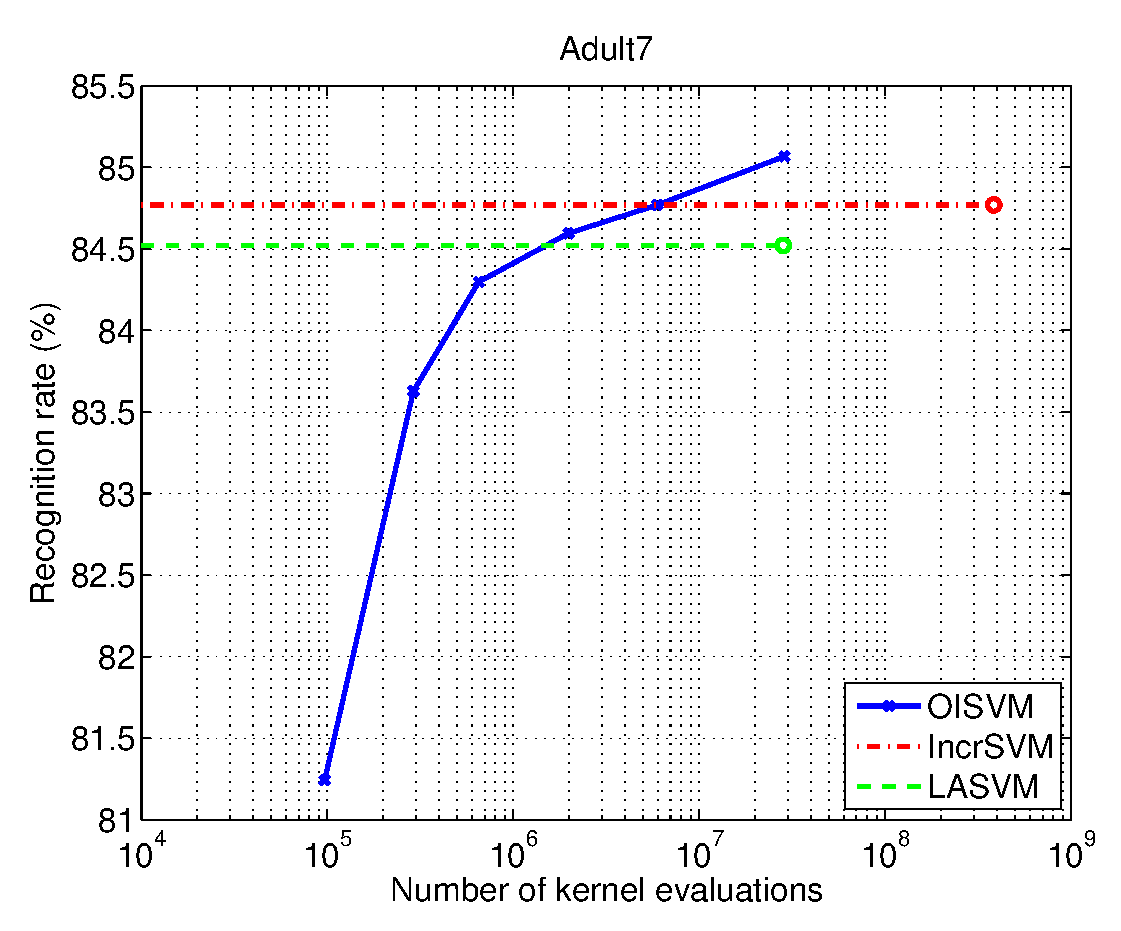
\includegraphics[width=0.48\linewidth]{figs/results/fig_a7a}} \\
  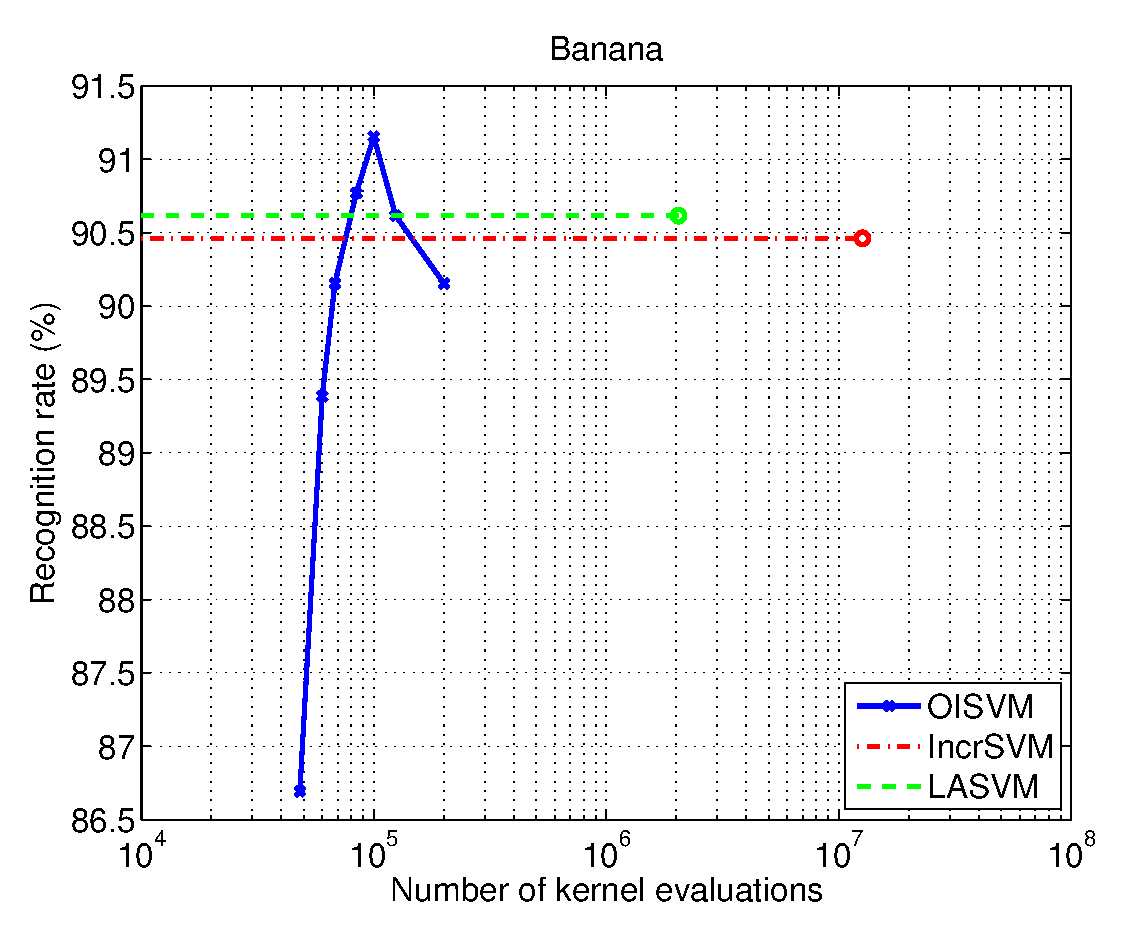
\includegraphics[width=0.48\linewidth]{figs/results/fig_banana} &
  \includegraphics[width=0.48\linewidth]{figs/results/fig_waveform}
  \end{tabular}
  \caption{Trade-off between accuracy and number of kernel evaluations of OISVM, IncrSVM and
  LASVM on 3 benchmarks.
  The OISVM curve is obtained plotting the number of kernel evaluations and the recognition rate at the end of the training, for each value of $\eta$. The number of kernel evaluations increases as $\eta$ decreases. 
  In LASVM and IncrSVM there is no parameter to trade accuracy for training speed, so only one
  point is shown.}
\label{fig:kernel_eval}
\end{figure*}
